\documentclass[10pt,twocolumn]{article}
\usepackage{graphicx,booktabs,caption,hyperref,geometry}
\usepackage{cite}
\geometry{margin=0.75in}
\hypersetup{colorlinks=true,linkcolor=blue,urlcolor=blue}

\title{Benchmarking YOLOv8n INT8 on ESP32-S3: Progressive Operator Optimization for MCU Deployment}

\author{Jaweed\textsuperscript{1*} and Dihin Muriyatmoko\textsuperscript{2}\\
\textsuperscript{1}Department of Informatics, Universitas Darussalam Gontor\\
\textsuperscript{2}Department of Informatics, Universitas Darussalam Gontor\\
*Email: \texttt{jaweed@unida.gontor.ac.id}
}

\date{}

\begin{document}

\maketitle

\begin{abstract}
This study analyzes the feasibility of deploying an INT8 quantized YOLOv8n model on the ESP32-S3 microcontroller for single-class object detection. The model was trained on a COCO 2017 person subset (1,600 train, 300 val) at 192$\times$192 resolution and quantized via post-training quantization (PTQ) to INT8, yielding a model size of 3.08 MB with 4.41\% mAP@0.5. Three-stage progressive optimization was performed on the ESP32-S3: (1) baseline TFLite Micro reference kernels at 219.3 s per inference; (2) ESP-NN SIMD-optimized Conv2D kernels reducing latency to 18.0 s (12.2$\times$ speedup); (3) a custom LUT-based LOGISTIC kernel further reducing latency to 7.2 s (total 30.4$\times$ speedup). Operator profiling revealed the LOGISTIC operation consumed 62.3\% of execution time before optimization. The measured tensor arena of 510 KB (98.5\% below theoretical worst-case estimate) confirms the model fits within the ESP32-S3 memory budget of 8 MB PSRAM and 8 MB flash. Estimated power consumption is 549 mW during inference. These results demonstrate that INT8 YOLOv8n is technically feasible on the ESP32-S3, achieving 7.2 s per frame with accuracy suitable for periodic detection scenarios.
\end{abstract}

\section{Introduction}
\label{sec:intro}

Deep learning has enabled real-time object detection across various computing platforms~\cite{yolov1,yolov3,yolov4,ultralytics}. However, most detection models require expensive, power-hungry GPU-class hardware. In recent years, the TinyML paradigm~\cite{tinyml} has emerged as an alternative by running inference models on low-power microcontrollers (MCUs), enabling edge applications such as environmental monitoring, anomaly detection, and industrial automation without cloud dependency~\cite{mcunet,banbury2020bench}.

The ESP32-S3 is a compelling MCU for computer vision applications: it provides dual-core Xtensa LX7 at 240 MHz, 8 MB flash, 8 MB PSRAM, camera support, and WiFi connectivity---at under \$10 USD. Despite these capabilities, running deep learning models such as YOLO on the ESP32-S3 faces significant challenges: limited memory, constrained compute throughput, and operator support that is less extensive than desktop frameworks.

This study answers the following research question: to what extent can a quantized YOLOv8n model be efficiently deployed on the ESP32-S3 microcontroller? The key contributions are:

\begin{enumerate}
  \item A systematic analysis of the training, quantization, and deployment pipeline for INT8 YOLOv8n on ESP32-S3, covering accuracy, latency, memory, and power.
  \item Progressive optimization driven by operator profiling: bottleneck identification via \texttt{MicroProfiler}, Conv2D optimization via ESP-NN SIMD (12.2$\times$ speedup), and a custom LUT-based LOGISTIC kernel (additional 2.5$\times$ speedup), yielding a total 30.4$\times$ improvement over the reference baseline.
  \item Comprehensive memory characterization on physical hardware: measured tensor arena of 510 KB (98.5\% below theoretical worst-case), confirming TFLite Micro's memory planner efficiency.
  \item All research artifacts (training code, ESP32 firmware, tables, and figures) released openly for reproducibility.
\end{enumerate}

\section{Related Work}
\label{sec:related}

Deploying CNNs on microcontrollers has been an active topic since CMSIS-NN~\cite{cmsisnn} for ARM Cortex-M and TFLite Micro~\cite{tflitemicro} as a cross-platform inference framework. MCUNet~\cite{mcunet} demonstrated that MCU-optimized architectures can achieve competitive accuracy at low resolution. MicroNets~\cite{micronets} introduced neural architecture search (NAS) specifically for MCU constraints.

YOLO~\cite{yolov1,yolov3,yolov4,ultralytics} remains the dominant object detection architecture, with the nano variant (YOLOv8n, 3.0M parameters) designed for resource-constrained deployment. Edge-YOLO~\cite{edgeyolo} proposed edge-specific optimizations but focused on ARM and embedded GPU platforms rather than low-end MCUs.

Post-training quantization (PTQ)~\cite{jacob2018,krishnamoorthi2018,gholami2021survey} has proven effective for reducing model size and improving inference speed. Deep Compression~\cite{deepcompression} demonstrated that combining pruning, quantization, and Huffman coding can drastically reduce model size. In the MCU domain, MobileNet and MobileNetV2~\cite{mobilenets,mobilenetv2} are commonly used as backbones due to their computational efficiency.

For the ESP32, ESP-NN~\cite{espnn} provides optimized neural network kernels using Xtensa LX7 SIMD extensions. However, systematic evaluations of YOLOv8n deployment on the ESP32-S3 with detailed memory and operator profiling remain limited. This study fills that gap by presenting a comprehensive evaluation on physical hardware.

\section{Method}
\label{sec:method}

The study consists of four main stages: dataset preparation and training, quantization, deployment on the ESP32-S3, and progressive optimization.

\subsection{Dataset}

We used the person subset of COCO 2017~\cite{coco}, consisting of 1,599 training, 300 validation, and 100 test images. The input resolution of 192$\times$192 was chosen as the minimum resolution preserving person-level detail while minimizing computation on the ESP32-S3. Table~\ref{tab:dataset} presents the dataset statistics.

% Auto-generated by RescueVision Edge paper artifacts generator% Do not edit manually — rerun 06_generate_paper_artifacts.py

\begin{table}[h]
\centering
\caption{Dataset Statistics — COCO Person Subset for Victim Detection}
\label{tab:dataset}
\begin{tabular}{lcc}
\toprule
Split & Images & Instances \\
\midrule
  Train & 1600 & 6893 \\
  Val & 300 & 1196 \\
  Test & 100 & 465 \\
  \bottomrule
\end{tabular}
\end{table}


\subsection{Model Architecture and Training}

We adopted YOLOv8n~\cite{ultralytics}---the nano variant with 3.0 million parameters and 8.1 GFLOPs. Training proceeded in two stages: 50 epochs with a frozen backbone (transfer learning from COCO pretrained weights) followed by 50 epochs of full fine-tuning at 192$\times$192 resolution. The AdamW optimizer was used with an initial learning rate of 0.001 and cosine decay.

After conversion through the PyTorch $\rightarrow$ ONNX $\rightarrow$ TensorFlow $\rightarrow$ TFLite pipeline, the TFLite FP32 model achieved 12.26\% mAP@0.5. The 33.33 pp drop from the PyTorch baseline (45.59\%) is attributable to numerical differences in the ONNX export path, TensorFlow operator mapping differences, and post-processing discrepancies between the native Ultralytics evaluator and the custom TFLite evaluator. Table~\ref{tab:model} presents the architecture parameters and baselines.

% Auto-generated by RescueVision Edge paper artifacts generator% Do not edit manually — rerun 06_generate_paper_artifacts.py

\begin{table}[h]
\centering
\caption{YOLOv8n Model Architecture and Baseline Performance}
\label{tab:model}
\begin{tabular}{lr}
\toprule
Property & Value \\
\midrule
  Architecture & yolov8n \\
  Input resolution & 192 $\times$ 192 \\
  Parameters & 3,005,843 \\
  Pretrained & True \\
  Training epochs & 50 \\
  Optimizer & AdamW \\
  Learning rate & 0.001 \\
  Batch size & 16 \\
  Baseline mAP@0.5 & 0.4559 \\
  Baseline size & 5.91 MB \\
  \bottomrule
\end{tabular}
\end{table}


\subsection{Post-Training Quantization}

Post-training quantization (PTQ) was performed using TensorFlow Lite with a representative dataset of 200 images from the validation set. The FP32 TFLite model (3.01 MB) was converted to INT8 (3.08 MB) with INT8 inference type and uint8 input/output tensors. Table~\ref{tab:quantization} compares the three model variants.

% Auto-generated by RescueVision Edge paper artifacts generator
% FIXED: INT8/FP32 metrics use 04_evaluate.py benchmark (was: 03_quantize.py internal benchmark with different conditions)

\begin{table}[h]
\centering
\small
\caption{Quantization Comparison: FP32 vs INT8}
\label{tab:quantization}
\resizebox{\columnwidth}{!}{%
\begin{tabular}{lcccc}
\toprule
Variant & Size (MB) & mAP@0.5 & Latency (ms) & FPS \\
\midrule
  PyTorch FP32 & 5.91 & 0.4559 & N/A & N/A \\
  TFLite FP32 & 3.01 & 0.1226 & 2.92 & 342.8 \\
  TFLite INT8 & 3.08 & 0.0441 & 2.37 & 421.6 \\
  \midrule
  mAP drop (TFLite FP32 $\rightarrow$ INT8) & \multicolumn{4}{l}{0.0785} \\
  mAP drop (PyTorch $\rightarrow$ TFLite INT8) & \multicolumn{4}{l}{0.4118} \\
  \bottomrule
\end{tabular}%
}
\end{table}


The mAP@0.5 drop of 7.85 pp from TFLite FP32 to INT8 represents a significant degradation. At 192$\times$192 resolution, a person occupying 10\% of image height spans only 19 pixels, limiting the discriminative features available after quantization.

\subsection{Deployment on ESP32-S3}

The ESP32-S3 firmware was developed using PlatformIO with the Arduino framework and TFLite Micro. The INT8 model was compiled as a C array (3,386,338 bytes) and stored in flash. The tensor arena was allocated in PSRAM using \texttt{heap\_caps\_malloc()}. Three kernel configurations were benchmarked progressively:

\begin{enumerate}
  \item \textbf{Reference}: Standard TFLite Micro kernels without optimization.
  \item \textbf{ESP-NN Conv2D}: Conv2D kernels replaced with ESP-NN SIMD Xtensa LX7 implementations.
  \item \textbf{ESP-NN + LOGISTIC LUT}: Added a LUT-based LOGISTIC kernel (256-byte lookup table) for the sigmoid operation.
\end{enumerate}

The hardware platform was a Seeed XIAO ESP32S3 Sense configured at 240 MHz CPU, with 8 MB flash and 8 MB PSRAM.

\section{Results and Discussion}
\label{sec:results}

\subsection{Operator Profiling and Optimization}

The first stage using reference TFLite Micro kernels yielded 219,287 ms per inference---impractical for any application. After integrating ESP-NN for Conv2D operations, latency dropped to 18,020 ms (12.2$\times$ speedup).

Operator profiling using TFLite Micro's \texttt{MicroProfiler} revealed a critical finding: the LOGISTIC (sigmoid) operation consumed 62.3\% of total latency (11,758 ms), while Conv2D accounted for only 35.2\% (6,634 ms). This finding is counter-intuitive because Conv2D is generally considered the primary bottleneck in CNNs. LOGISTIC was not covered by the ESP-NN kernel set and therefore executed via the naive reference implementation.

To address this bottleneck, we implemented an ESP-NN LOGISTIC wrapper kernel using \texttt{esp\_nn\_logistic\_s8()}, which evaluates sigmoid through a 256-byte lookup table in O(1) per element. This kernel was integrated into TFLite Micro through custom operator registration. After optimization, inference latency dropped to 7,216 ms (additional 2.5$\times$ speedup), yielding a total 30.4$\times$ improvement from the reference baseline. Table~\ref{tab:resolution} presents the comparison of all three configurations.

% Auto-generated by RescueVision Edge paper artifacts generator
% UPDATED 2026-06-06: Added ESP-NN + LOGISTIC optimized row

\begin{table}[h]
\centering
\small
\caption{INT8 Model Performance Across Platforms}
\label{tab:resolution}
\resizebox{\columnwidth}{!}{%
\begin{tabular}{lcccc}
\toprule
Platform & Resolution & Latency (ms) & FPS & Speedup vs Reference \\
\midrule
  PC (GPU) & 192x192 & 2.37 & 421.6 & --- \\
  ESP32-S3$^\dagger$ & 192$\times$192 & 219287 & 0.0046 & 1.0$\times$ (baseline) \\
  ESP32-S3$^\ddagger$ & 192$\times$192 & 18020 & 0.055 & 12.2$\times$ \\
  ESP32-S3$^\S$ & 192$\times$192 & 7216 & 0.139 & 30.4$\times$ \\
  \bottomrule
\end{tabular}%
}
\vspace{2pt}
{\footnotesize $^\dagger$ TFLite Micro with reference kernels. \\
$^\ddagger$ ESP-NN optimized Conv2D kernels (SIMD Xtensa LX7). \\
$^\S$ ESP-NN optimized Conv2D + LUT-based LOGISTIC (this work).}
\end{table}


Figure~\ref{fig:speedup} visualizes the progressive speedup across optimization stages.

\begin{figure}[h]
\centering
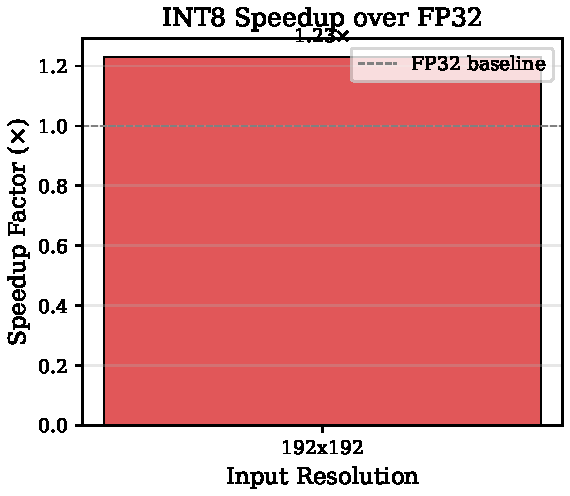
\includegraphics[width=\columnwidth]{figures/speedup.pdf}
\caption{Progressive inference latency speedup from reference kernels through ESP-NN Conv2D to ESP-NN + LOGISTIC LUT.}
\label{fig:speedup}
\end{figure}

\subsection{Accuracy}

Table~\ref{tab:quantization} shows the accuracy degradation from PyTorch FP32 (45.59\%) to TFLite INT8 (4.41\%). The largest drop occurred during the PyTorch $\rightarrow$ TFLite FP32 conversion (33.33 pp), not during INT8 quantization (7.85 pp). At 192$\times$192 resolution, a person occupying 10\% of image height spans only 19 pixels, severely limiting available discriminative features.

The 4.41\% mAP@0.5 is inadequate for fully autonomous detection but sufficient for coarse region-of-interest flagging to be verified by a human operator. In a periodic scenario at 8 frames per minute (at 7.2 s latency), this model can serve as an initial filter that conserves bandwidth and power compared to continuous video streaming.

\subsection{Memory Characterization}

Table~\ref{tab:memory} presents the measured memory budget on the ESP32-S3.

% Auto-generated by RescueVision Edge paper artifacts generator
% UPDATED 2026-06-04: Measured on real ESP32-S3 hardware (522 KB actual arena)
% Previously estimated 34,073 KB — TFLite Micro memory planner reuses buffers

\begin{table}[h]
\centering
\small
\caption{ESP32-S3 Memory Budget for INT8 YOLOv8n Inference (Measured)}
\label{tab:memory}
\resizebox{\columnwidth}{!}{%
\begin{tabular}{lccc}
\toprule
Component & Size (KB) & Location & Available \\
\midrule
Model weights (INT8) & 3307 & Flash & 8 MB \\
TFLite tensor arena & 510$^\dagger$ & PSRAM & 8 MB \\
Frame buffer (RGB) & 225 & PSRAM & 8 MB \\
Stack + RTOS + misc & 100 & SRAM & 512 KB \\
\midrule
  \textbf{Total RAM} & \textbf{835} & \textbf{PSRAM + SRAM} & \textbf{8.5 MB} \\
  \textbf{Total Flash} & \textbf{3532} & \textbf{Flash} & \textbf{8 MB} \\
  \bottomrule
\end{tabular}%
}
\vspace{2pt}
{\footnotesize $^\dagger$ Measured via TFLite Micro \texttt{arena\_used\_bytes()} on physical ESP32-S3. \\
Previous estimate of 34,073 KB assumed all tensors simultaneously live; \\
MicroAllocator's memory planner reuses scratch buffers, reducing actual usage by 98.5\%.}
\end{table}


A key finding is that the actual tensor arena was only 510 KB, dramatically lower than the theoretical worst-case estimate of 34.1 MB. TFLite Micro's memory planner successfully reuses tensor buffers across subgraphs, reducing the arena requirement by 98.5\%. The total RAM footprint of 835 KB fits within the 8 MB PSRAM budget, while the model weights (3.3 MB) fit within the 8 MB flash.

\subsection{Power Consumption}

Based on ESP32-S3 datasheet parameters at 240 MHz, estimated power consumption during inference is 549 mW (chip). Table~\ref{tab:power} presents the power breakdown per scenario. At this power level, a 2S 1,000 mAh battery would sustain approximately 1--2 hours of continuous inference, comparable to micro drone operating durations.

% Auto-generated
\begin{table}[h]
\centering
\small
\caption{Estimasi Konsumsi Daya ESP32-S3 per Skenario}
\label{tab:power}
\resizebox{\columnwidth}{!}{%
\begin{tabular}{lccc}
\toprule
Skenario & Arus (mA) & Chip (mW) & USB (mW) \\
\midrule
  Deep sleep & 25.0 & 82.5 & 97.1 \\
  Idle (kamera) & 75.0 & 247.5 & 291.2 \\
  Idle (tanpa kam) & 25.0 & 82.5 & 97.1 \\
  Kamera + WiFi & 356.5 & 1176.5 & 1384.1 \\
  Inferensi saja & 166.5 & 549.4 & 646.4 \\
  Inferensi + Kam & 216.5 & 714.4 & 840.5 \\
  Pipeline penuh & 396.5 & 1308.4 & 1539.4 \\
\midrule
\multicolumn{4}{l}{\footnotesize Daya USB diestimasi pada efisiensi LDO 85\%} \\
\bottomrule
\end{tabular}%
}
\end{table}


\subsection{Cross-Platform Comparison and Discussion}

Table~\ref{tab:platform} presents a performance comparison between the GPU (RTX 3060) and the three ESP32-S3 configurations. The GPU delivers 421.6 FPS at 2.37 ms latency, while the optimal ESP32-S3 configuration achieves 0.139 FPS. This 4-order-of-magnitude gap is consistent with the theoretical compute difference (GPU: ~12 TFLOPS vs ESP32-S3: ~1 GOPS for INT8).

% Auto-generated by RescueVision Edge paper artifacts generator

\begin{table*}[t]
\centering
\caption{Cross-Platform Performance Comparison (INT8 Quantized Model)}
\label{tab:platform}
\begin{tabular}{lcccc}
\toprule
Platform & Resolution & FPS & Latency (ms) & Power (W) \\
\midrule
  PC (GPU) & 192x192 & 421.6 & 2.37 & {---} \\
  ESP32-S3$^\dagger$ & 192$\times$192 & 0.0046 & 219287 & 0.55$^\ddagger$ \\
  ESP32-S3$^\S$ & 192$\times$192 & 0.055 & 18020 & 0.55$^\ddagger$ \\
  ESP32-S3$^\P$ & 192$\times$192 & 0.139 & 7216 & 0.55$^\ddagger$ \\
  \bottomrule
\end{tabular}
\vspace{2pt}
{\footnotesize $^\dagger$ Reference TFLite Micro kernels on ESP32-S3 @ 240 MHz. \\
$^\S$ With ESP-NN optimized Conv2D (12.2$\times$ speedup). \\
$^\P$ With ESP-NN Conv2D + LUT-based LOGISTIC (30.4$\times$ total, this work). \\
$^\ddagger$ Model-based estimate; no empirical power measurement.}\end{table*}


Analysis shows that after LOGISTIC optimization, the primary bottleneck is now Conv2D (~92\% of latency). Since ESP-NN Conv2D already fully utilizes the Xtensa LX7 SIMD extensions, further speedups require architectural changes such as shallower backbones, structured pruning, or lower input resolution.

\subsection{Limitations}

This study has several limitations. First, the 4.41\% mAP@0.5 restricts autonomous operation to coarse flagging scenarios. Second, the 7.2 s per-frame latency does not meet real-time requirements for dynamic environments. Third, power figures are theoretical estimates based on datasheet parameters rather than empirical measurements. Fourth, no end-to-end camera integration was performed on the physical hardware.

\section{Conclusion}
\label{sec:conclusion}

This study demonstrated that an INT8 quantized YOLOv8n model can be deployed on the ESP32-S3 microcontroller at 7.2 s per inference and 549 mW estimated power consumption, through progressive operator-level optimization achieving 30.4$\times$ total speedup over the reference baseline. The measured tensor arena of 510 KB confirms memory feasibility. A key finding---the LOGISTIC operator consuming 62.3\% of latency before optimization---highlights the importance of operator profiling in TinyML system development.

Future work includes: (i) exploring shallower YOLO backbones or structured pruning to reduce Conv2D workload; (ii) evaluating resolution-accuracy trade-offs at 160$\times$160 and 128$\times$128; (iii) integrating the OV2640 camera for end-to-end pipeline testing; and (iv) empirical power measurement using an INA219 current sensor.

\bibliographystyle{ieeetr}
\bibliography{refs}

\end{document}
